\chapter{Arrays: scalars, vectors and matrices}
\thispagestyle{fancy}
\label{ch:arrays}

Besides using \MATLAB{} as a common calculator, it is possible to perform calculations on entire datasets. These variables must be stored in the workspace and addressed by their variable name. Variables are stored in the \MATLAB{} workspace as arrays. The four main array types that we will use are:



\begin{description}
\item [Scalar\index{scalar}] 1x1 array containing one value
\item [Vector\index{vector}] a row or column array (1xM or Mx1 array) containing M values
\item [Matrix\index{matrix}] a 2-dimensional array (e.g. a map)
\item [Multi-dimensional arrays\index{multi-dimensional arrays}] e.g. a 5x2x3 array containing 30 values
\end{description}

\hintbox{You can retrieve the size of an array by issuing a {\tt size(X)}\index{size@\texttt{size}} command, where {\tt X} represents the array that you want to know the size of.}



\section{Data types\index{data types} and array classes\index{array classes}}

\MATLAB{} arrays can contain three different data types: integer\index{integer}, floating point\index{floating point}, and character\index{character} data. 

\hintbox{A character variable is often referred to as a `string'\index{string}, especially when it contains more than one character.}

\noindent A description of different data types and the array classes in which they are stored is given in Table~\ref{tab:array-classes}.

\begin{table}[ht]
\caption{Array classes}
\label{tab:array-classes}
\vspace{-0.5em}
\centering
\begin{tabular}{|p{2cm}|l|p{3cm}|p{2cm}|}
\hline
\textbf{Data type}&\textbf{Examples}&\textbf{Description}&\textbf{Array class}\\
\hline
Integer&\verb#-2 -5 -8 0 2 34 221#&(+/-) Whole numbers&Double array\\
\hline
Floating point&\verb#3.2232 �8.323 5823.22#& (+/-) Fractional numbers&Double array\\
\hline
Character&\verb#y L \ = ] - K , u ;#&ASCII text characters&Character array\\
\hline
\end{tabular}
\end{table}



\section{Creating arrays}

Besides using existing datasets for analysis, it is important to be able to create and manipulate your own arrays within the \MATLAB{} environment. This can vary from creating a simple vector with an increasing value from 1 to 365 to serve as a time indicator for a certain process to complex 4-D arrays with certain parameters at a place in space (X, Y, Z) that change over time. The value of each position in an array can then be manipulated to simulate a process. These operations can be performed on complete arrays or selected cells.

 
\begin{action}
Type 
\end{action}
\prompt{A = [1,2,3;4,5,6]}
\noindent \verb#A# is now present in the workspace as a 2x3 double array. When declaring arrays other than scalars, the array contents must be in brackets \verb#[ ]#. If you take a closer look at the output that \MATLAB{} returns, you'll see that you just made an array with 2 rows and 3 columns. 
\hintbox{Commas ({\tt,}) serve as column delimiters, and semicolons ({\tt;}) are row delimiters.}
\noindent There are several ways to create vectors:
\begin{action}
Type 
\end{action}
\prompt{k = [1:1:9]}
\noindent press \guitext{Enter} and interpret the result.

\begin{action}
Type 
\end{action}
\prompt{m = [21:-2:13]}
\noindent press \guitext{Enter} and interpret the result. As you can see, the syntax of this command is \verb#[#minimum\verb#:#increment\verb#:#maximum\verb#]#.

\begin{action}
Generate an array starting with 10.2, decreasing with 0.3 and ending at 6.0.
\end{action}

\begin{action}
As simple as you can generate 1-D arrays, you can also make 2-D arrays; type 
\end{action}
\prompt{F = [-10:1:10;40:-1:20]}
\noindent and interpret the result.


\begin{action}
Type 
\prompt{G = [-5:1:15;8:-0.5:1.0]}
\noindent and interpret the error.
\end{action}
\begin{action}
Once an array contains one of the three data types, it cannot contain another data type as well. Type 
\end{action}
\prompt{H = [1,2,3;\squote{PiM}]}
\noindent and interpret the result.

 
\begin{action}
Now type 
\end{action}
\prompt{I = [1,2,3,4;\squote{PiM}]}
\noindent and interpret the error.

\section{Manipulating arrays by their subscripts\index{subscripts} and indices\index{index}\index{indices}}

Elements of arrays are identified by their positions in the array. So\dots
\vspace{0.5em}
\prompt{F(2,6)}
\noindent returns 35. This is the value of the element in the second row and the sixth column in matrix \verb#F#. 

Elements can also be identified by their index. The index is a counter that starts at the first row and first column, then continues down in the first column and then takes next column. To clarify the difference between indices and subscripts, take a closer look at the tables below:



\begin{table}[ht]
\caption{Array elements identified by subscripts}
\label{tab:subscripts}
\vspace{-0.5em}
\centering
\begin{tabular}{|p{0.75cm}|p{0.75cm}|p{0.75cm}|}
\hline
(1,1)&(1,2)&(1,3)\\
\hline
(2,1)&(2,2)&(2,3)\\
\hline
(3,1)&(3,2)&(3,3)\\
\hline
\end{tabular}
\end{table}

\begin{table}[ht]
\caption{Array elements identified by indices}
\label{tab:indices}
\vspace{-0.5em}
\centering
\begin{tabular}{|p{0.75cm}|p{0.75cm}|p{0.75cm}|}
\hline
(1)&(4)&(7)\\
\hline
(2)&(5)&(8)\\
\hline
(3)&(6)&(9)\\
\hline
\end{tabular}
\end{table}


\begin{action}
Retrieve the value of the element denoted by subscript 2,1 in matrix {\tt A}. What value do you expect?
\prompt{A(2,1)}
\end{action}

\hintbox{Parenthesis symbols {\tt( )} are used to point to elements of an array, in contrast to the {\tt[ ]} square brackets that are used to assign values to the array.}

\begin{action}
What is the index of the value 23 in the matrix {\tt F}? And what are the subscripts?
\end{action}

\begin{action}
Alter the values in a matrix by calling their indices or subscripts and assigning a new value: 
\end{action}
\prompt{F(20) = -40}
\noindent Now check what has changed in the matrix {\tt F}.

\vspace{1em}
\noindent You have now altered one array element of matrix {\tt F} by using a scalar as index. You can also change more than one array element of {\tt F}, at the same time, by using an index vector instead of just one index scalar. 

\begin{action}
Carefully interpret the sentence above and (try to) change the array elements of {\tt F} to �50 where the index is equal to one of the elements of the vector {\tt IndVec}, when given: 
\end{action}
\prompt{IndVec = [3,15,2,8,19]}

\begin{action}
Can you this do this in a single command? 
\end{action}
 

\section{Matlab demonstrations}

Maybe this is a good moment to take a break for a while and to have a look at some demonstrations for 10--15 minutes, as \MATLAB{} has an extensive `{\tt demo}'\index{demo@\texttt{demo}} function. When you see what you can do with \MATLAB{}, you have a better reference while studying this text and while doing the exercises. Select one or two of the most instructive demos and share these with your neighbors. 

\begin{action}
Start \MATLAB{} demonstrations by typing {\tt demo} on the \MATLAB{} command line. 
\end{action}

\noindent The help documentation window that pops up consists of two panes. Read the contents of the right pane. After that, try expanding one of the menu tree items in the left pane, for example \MATLAB{} \ding{217} graphics (see Figure~\ref{fig:demo}).

\begin{figure}[!ht]
  \centering
    \fbox{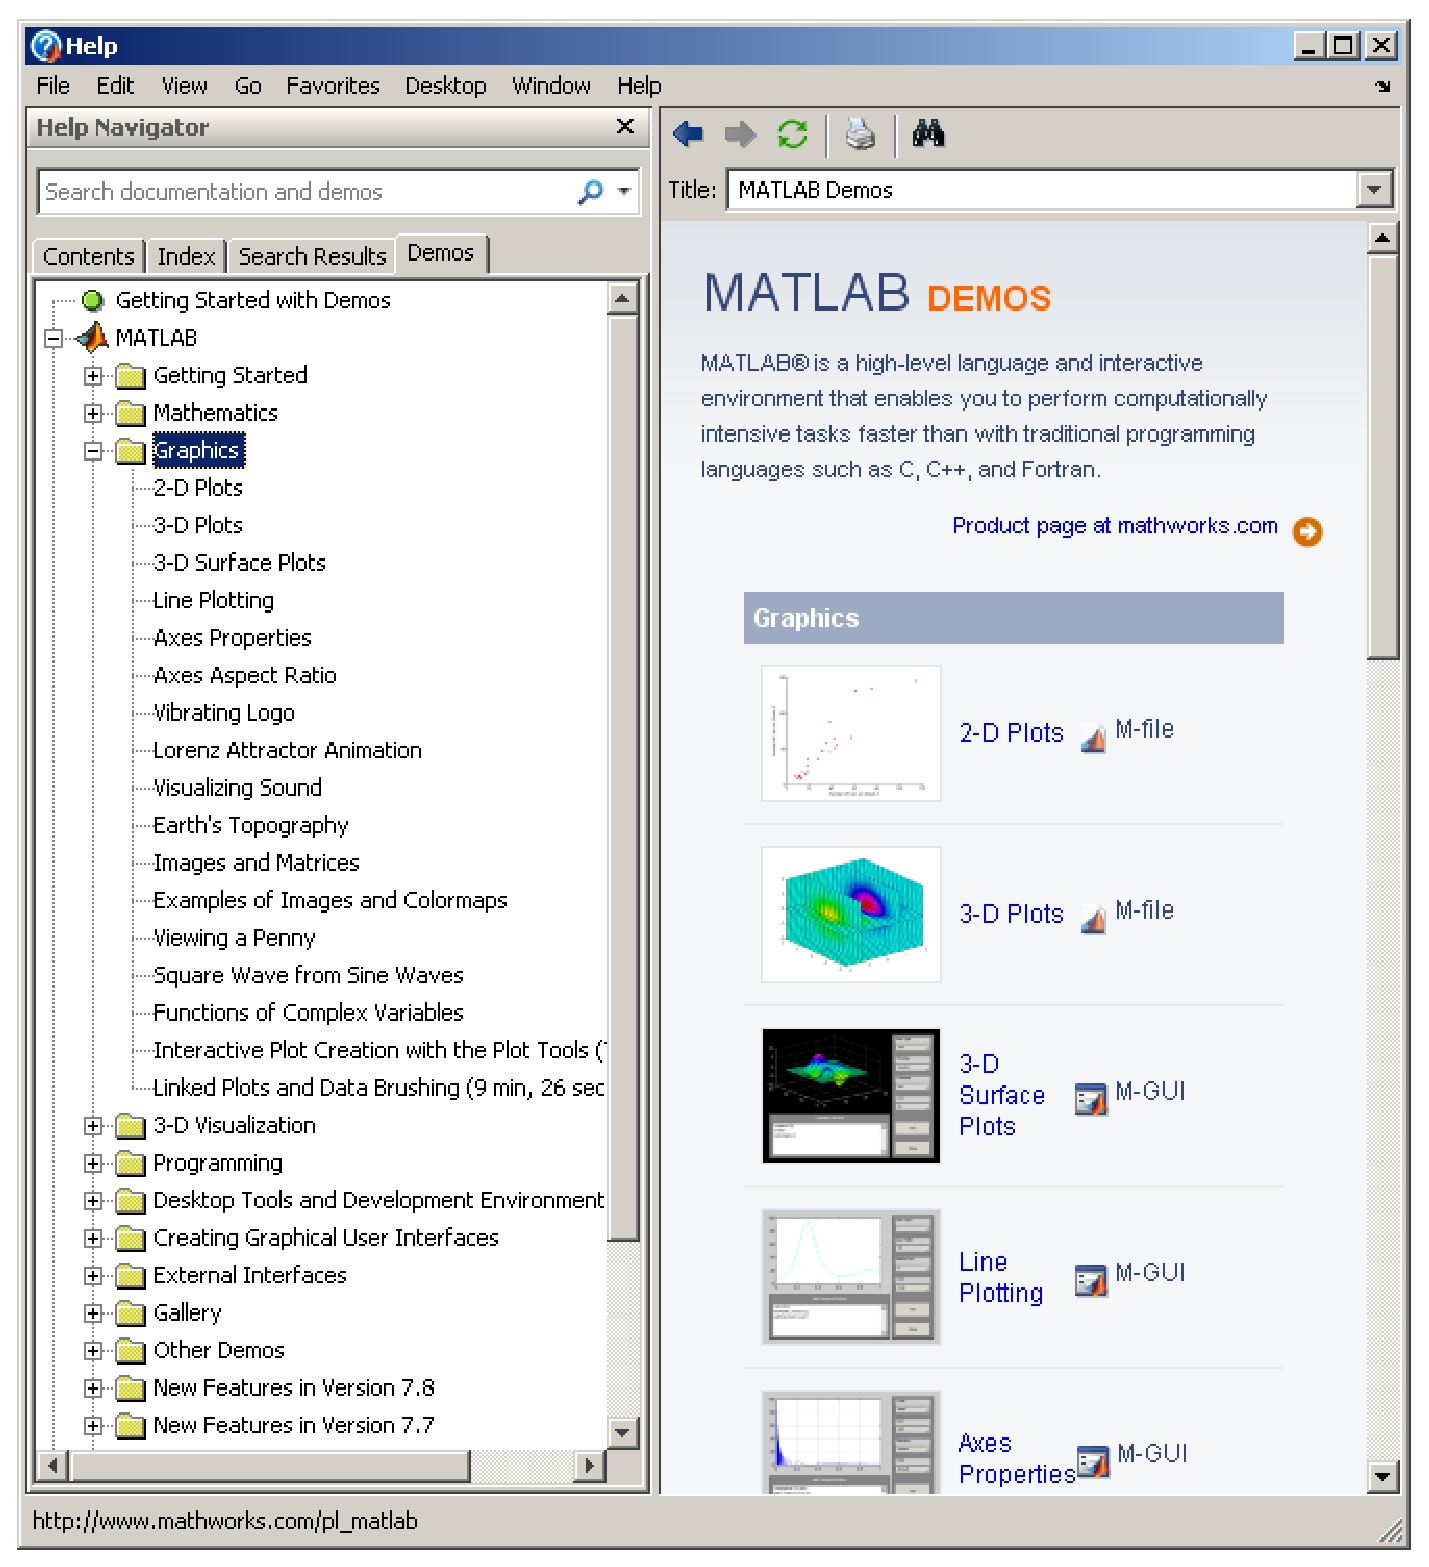
\includegraphics[width=1.0\textwidth]{./../eps/demo.eps}}
  \caption{\MATLAB{} demonstrations.}
  \label{fig:demo}
\end{figure}



\section{Arithmetic operations on matrices and vectors}

Just as you can perform calculations on scalars (as we did in the exercise with the precipitation), you could perform calculations on larger arrays as well. Some examples are outlined below:

\subsection{Multiplication of a scalar with a 2-D array}

\begin{equation}
\label{eq:scalar-matrix-multiplication}
5\ast
\left[ 
\begin{array}{rrr}
4&5&2\\
1&9&0\\
1&5&5\\
\end{array}
\right]
=
\left[
\begin{array}{rrr}
20&25&10\\
5&45&0\\
5&25&25\\
\end{array}
\right]
\end{equation}

\noindent Or, in \MATLAB{}:
\prompt{A = 5}
\prompt{B = [4,5,2;1,9,0;1,5,5]}
\prompt{C = A * B}


\subsection{Addition of 2-D arrays}


\begin{equation}
\label{eq:addition-2D}
\left[ 
\begin{array}{rrr}
-1&2&0\\
2&-3&1\\
-4&0&5\\
\end{array}
\right]
+
\left[ 
\begin{array}{rrr}
4&5&2\\
1&9&0\\
1&5&5\\
\end{array}
\right]
=
\left[
\begin{array}{rrr}
3&7&2\\
3&6&1\\
-3&5&10\\
\end{array}
\right]
\end{equation}


\noindent Or, in \MATLAB{}:
\prompt{D = [-1,2,0;2,-3,1;-4,0,5]}
\prompt{B = [4,5,2;1,9,0;1,5,5]}
\prompt{E = D + B}


\subsection{Multiplication of 2-D arrays (`dot-product')}


\begin{equation}
\label{eq:multiplication-2D-dot-product}
\left[ 
\begin{array}{rrr}
3&1&7\\
8&4&6\\
\end{array}
\right]
\bullet
\left[ 
\begin{array}{rrr}
4&5\\
2&1\\
9&0\\
\end{array}
\right]
=
\left[
\begin{array}{rrr}
77&16\\
94&44\\
\end{array}
\right]
\end{equation}


\noindent Or, in \MATLAB{}:
\prompt{F = [3,1,7;8,4,6]}
\prompt{G = [4,5;2,1;9,0]}
\prompt{H = F * G}

\noindent In general, elements of \verb#H# are calculated using:
\begin{equation}
\label{eq:matrix-multiplication}
H(r,c) = \sum_{k=1}^{nElems}{F(r,k)\times{}G(k,c)}
\end{equation}
in which $r$ is the row number, $c$ is the column number, $nElems$ is the number of columns in $F$ (or, equivalently, the number of rows in $G$). For example:

\noindent \begin{array}{cccccccccccccl}
H(1,1)& = &F(1,1)&*&G(1,1)&+&F(1,2)&*&G(2,1)&+&F(1,3)&*&G(3,1)&=\\ 
&&3&*&4&+&1&*&2&+&7&*&9&=77\\ 
\end{array}

\noindent Note that \verb#F * G# returns a different result than \verb#G * F#.

\subsection{Multiplication of 2-D arrays (element-by-element)}

\begin{equation}
\label{eq:multiplication-2D-product}
\left[ 
\begin{array}{rrr}
3&1&7\\
8&4&6\\
5&3&4\\
\end{array}
\right]
\ast
\left[ 
\begin{array}{rrr}
4&5&2\\
1&9&0\\
1&5&5\\
\end{array}
\right]
=
\left[
\begin{array}{rrr}
12&5&14\\
8&36&0\\
5&15&20\\
\end{array}
\right]
\end{equation}

\noindent In \MATLAB{}, if you want to calculate the product of \verb#A# and \verb#B# element-by-element, you need to use a period sign (`\verb#.#') between the first matrix and the operator:

\prompt{J = [3,1,7;8,4,6;5,3,4]}
\prompt{B = [4,5,2;1,9,0;1,5,5]}
\prompt{K = J .* B}
\noindent so that elements of K are calculated using $K(r,c) = J(r,c)*B(r,c)$. Note that there is no difference between $J * B$ and $B * J$, since the array elements are multiplied on an element-by-element basis anyway.

\begin{action}
Is it possible to calculate \verb#M*N# if both \verb#M# and \verb#N# are arrays of size 3x2? Why or why not? If you don't know, just try it out in the Command Window! 
\end{action}
\begin{action}
Same question for \verb#M.*N#
\end{action}


\vspace{2em}

\noindent Recall the precipitation example in Chapter \ref{ch:getting-started}. In that example, the precipitation had been measured for a different period in each city:
\begin{table}[ht]
\caption{Precipitation records}
\label{tab:precipitation-records}
\vspace{-0.5em}
\centering
\begin{tabular}{|l|l|l|}
\hline
\textbf{City}&\textbf{Period}&\textbf{Mean Daily Precipitation}\\
\hline
Groningen&12&2.33\\
\hline
Utrecht&27&2.12\\
\hline
Maastricht&18&1.92\\
\hline
\end{tabular}
\end{table}



\begin{action}
Create two 3x1 arrays, \verb#Period# and \verb#MDP# (Mean Daily Precipitation), that contain the measuring period (in days) and mean daily precipitation (in mm/day), respectively for the three Dutch cities. Use matrix operations to calculate a 3x1 array \verb#TP# with total precipitation (in mm) for every city during their respective measuring periods.
\end{action}



\section{Concatenation}
\label{ch:concatenation}
It can be useful to combine separate arrays with related data into one array. This is called concatenation\index{concatenation}.

\begin{action}
Type:
\end{action}
\prompt{A = 5}
\prompt{B = 6}
\prompt{C = [A,B]}
\noindent and check what \verb#C# contains.

\begin{action}
What is the difference between typing \verb#C = [A;B]# instead of \verb#C = [A,B]#?
\end{action}

\begin{action}
It is also possible to add a new row and/or column to an existing array:
\end{action}
\prompt{D = 1}
\prompt{E = 3}
\prompt{F = 4}
\prompt{G = [D,2;E,F;C]}


\begin{action}
Concatenate the three arrays \verb#Period#, \verb#MDP#, and \verb#TP# into one array named \verb#PrecInfo#.
\end{action}


\begin{action}
Take 15 minutes to review what you have learned so far in chapters \ref{ch:getting-started} and \ref{ch:arrays}.
\end{action}

\project{Columbia River}
\label{pr:columbia}
\noindent In this exercise you will use much more data than can be typed quickly, so you will load the data from a file. You also cannot display all results as numbers on the screen, so you will learn some of the basics of making graphical presentations.

Suppose that you have measured the stream water velocity in the Columbia River. This data is stored in a file titled `columbia\_river.mat'.

\begin{action}
Go to \url{http://blackboard.ic.uva.nl} and download the file \mbox{`pim\_files.zip'}. This zipfile contains all the files that you will need during this course. Unzip it to your network drive or usb-memory. It contains the folder structure displayed in Figure~\ref{fig:folder-structure}. As you can see, each chapter has its own folder. Some folders contain subfolders labeled according to the project number.
\end{action}

\begin{figure}[!ht]
  \centering
    \fbox{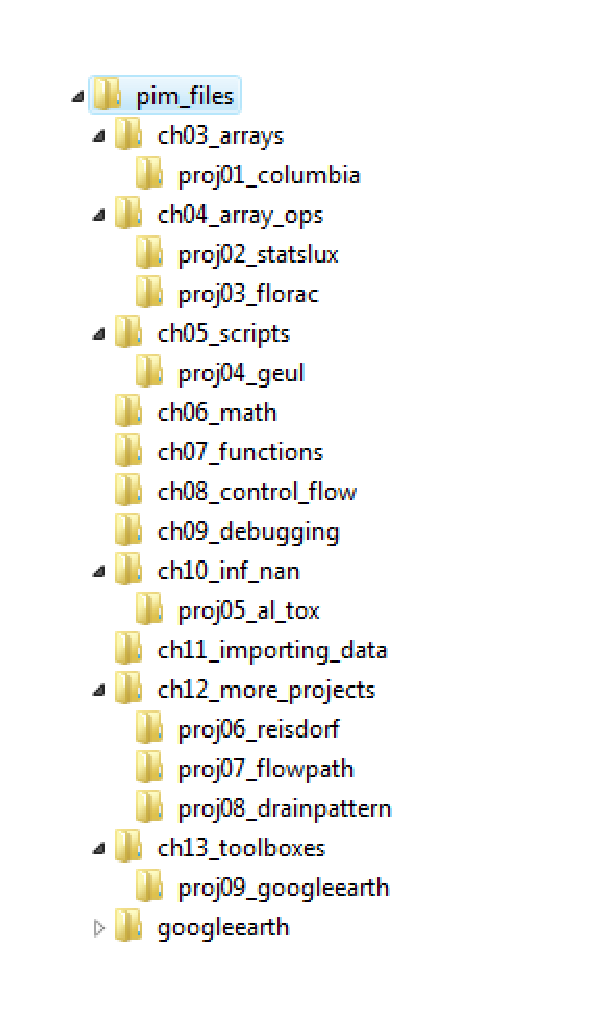
\includegraphics[width=0.33\textwidth]{./../eps/folder-structure}}
  \caption{Folder structure.}
  \label{fig:folder-structure}
\end{figure}



\begin{action}
Set your work directory to `\textbackslash{}ch03\_arrays\textbackslash{}proj01\_columbia'. The file `columbia\_river.mat' contains stream velocity data from the Columbia River in Oregon, averaged over total depth\footnote{Data from Savini and Bodhaine (1971) US Geological Survey}.
\end{action}

\hintbox{Make it a habit to clear your workspace with the {\tt clear} command before you start a new exercise. Doing this makes your calculations faster and will help diminish the interference from unnecessary variables. 
}

\begin{action}
Load \mbox{`columbia\_river.mat'} into the workspace (a *.mat file is a binary file, it can contain multiple variables):
\end{action}
\prompt{load columbia\_river.mat}\index{load@\texttt{load}}


\begin{action}
Check the variables you loaded for Columbia River in the workspace. Check the size and the values for these arrays in the \guitext{Workspace} window.
\end{action}


\hintbox{A calculation statement that does not end with a semicolon ( {\tt ;} ) echoes the answer to the screen. This may be undesirable if you are working with large matrices, because you don't want these matrices scrolling endlessly on your screen. A statement with a semicolon carries out the same task but does not echo the result to the screen. Display the array {\tt Sensor\_1} from the Columbia River project and then again using the semicolon:
\vspace{0.25em}
 
\prompt{Sensor\_1}
\prompt{Sensor\_1;}

}%close hintbox

\section{Simple plotting}
\noindent \MATLAB{} can display all kinds of graphs. An easy-to-use visualization tool is the \verb#plot(X,Y)#\index{plot@\texttt{plot}} command. This command plots the elements of a vector \verb#X# on the x-axis versus the values of a vector \verb#Y# on the y-axis (see Figure~\ref{fig:plotxy}).




\begin{figure}[ht]
\begin{minipage}{0.65\textwidth}
\centering
\includegraphics[width=\textwidth]{./../eps/plotxy}
\end{minipage}
~\hfill~
\begin{minipage}{0.25\textwidth}
\centering
\begin{tabular}{|c|c|}
\hline
\textbf{X}&\textbf{Y}\\
\hline
9.46&0.95\\
11.17&0.23\\
15.69&0.61\\
18.95&0.49\\
20.71&0.73\\
\hline
\end{tabular}
\end{minipage}
\caption{{\tt plot} with X and Y coordinates specified.}
\label{fig:plotxy}
\end{figure}



If no X-vector is specified (\verb#plot(Y)#), \MATLAB{} visualizes the data from vector \verb#Y# versus its indexes (see Figure~\ref{fig:ploty} on page \pageref{fig:ploty}).



\begin{figure}[ht]
\begin{minipage}{0.65\textwidth}
\centering
\includegraphics[width=\textwidth]{./../eps/ploty}
\end{minipage}
~\hfill~
\begin{minipage}{0.25\textwidth}
\centering
\begin{tabular}{|c|c|}
\hline
\textbf{X}&\textbf{Y}\\
\hline
1&0.95\\
2&0.23\\
3&0.61\\
4&0.49\\
5&0.73\\
\hline
\end{tabular}
\end{minipage}
\caption{{\tt plot} with only Y coordinates specified explicitly.}
\label{fig:ploty}
\end{figure}

\begin{action}
Display the data of \verb#Sensor_1# using the plot command.
\end{action}
\prompt{plot(Sensor\_1)}


\noindent This plot contains the time on the horizontal axis and the stream water velocity on the vertical axis. To indicate what the figure you created is about, we need to give it a title. This is done using the {\tt title(\squote{s})}\index{title@\texttt{title}} command. The variable \verb#s# represents the text to be used in the title. Don't forget to put this text string inside single quotation marks, otherwise \MATLAB{} will return an error. 

\begin{action}
Give the figure a title: `Columbia River, near Priest River Dam'. If you are not sure how to assign titles to figures, you can consult the \verb#doc#\index{doc@\texttt{doc}} function (see the tip below). 
\end{action}


\noindent Just as we can put a title on a figure, it's also possible to assign text labels to the axes. This is done using the commands {\tt xlabel}\index{xlabel@\texttt{xlabel}} and {\tt ylabel}\index{ylabel@\texttt{ylabel}}.

\hintbox{There are different ways to get help in \MATLAB{}. By far the most important and easy-to-use is the {\tt doc} command. For instance try typing {\tt doc mean} to read about how to use \MATLAB{}'s built-in function to calculate the mean of an array. Other commands that are sometimes helpful are: {\tt help}\index{help@\texttt{help}} and {\tt lookfor}\index{lookfor@\texttt{lookfor}}.}


\begin{action}
Consult the \verb#doc# function to find out how to assign labels to the x and y axes. Label the x-axis `Time (minutes)' and the y-axis `Velocity (m/s)'.
\end{action}

\begin{action}
Type 
\end{action}
\prompt{legend(\squote{velocity [m/s]})}\index{legend@\texttt{legend}}
\noindent to create a legend for the stream velocity plot of the Columbia River.

\vspace{1em}
\noindent There is a problem: previous experience with this sensor shows that a stream velocity correction is needed for this stream segment: 

\begin{equation}
TV1 = -0.18 + 0.987 * MV1 
\end{equation}
where $TV1$ is the true stream velocity and $MV1$ is the velocity as recorded by sensor~1.

\begin{action}
Calculate the true stream velocity of the river, measured with sensor~1.
\end{action}

\noindent After 66 measurements, unfortunately sensor~1 broke down. Luckily, a backup sensor, sensor~2, was available at the same stream location. The variable \verb#Sensor_2# contains the data from this sensor. However, this one also needs a correction: 
\begin{equation}
TV2 = -0.02 + 1.002 * MV2
\end{equation}
where $TV2$ is the true stream velocity and $MV2$ is the velocity as recorded by sensor~2.


\begin{action}
Correct the second data set (\verb#Sensor_2#) with this algorithm and append the corrected sensor~2 data to the first 66 measurements gathered at sensor~1 into a new merged stream data array, called \verb#Columbia#. Plot the result. Try to plot the 2~variables \verb#Sensor_1# and \verb#Sensor_2# with different colors. Consult the help documentation if necessary.
\end{action}

\begin{action}
Print the figure you created for your Columbia River stream velocities.
\end{action}

\begin{action}
Save the merged and corrected data array into a binary file by typing:
\end{action}
\prompt{save merged\_sensors.mat Columbia}\index{save@\texttt{save}}
\noindent which means: save the content of the variable Columbia in the binary file `merged\_sensors.mat'.

\projectfooter{}



